\section{Tính toán chuẩn \hinf}
Trong phần này, hai thuật toán để tìm chuẩn \hinf của một hệ thống điều khiển tuyến tính được trình bày. Xấp xỉ chuẩn \hinf của một hệ thống yêu cầu tính toán supremum của phản hồi trên tất cả tần số, do đó việc sử dụng quy trình lặp lại là bắt buộc. Mỗi liên hệ giữa chuẩn \hinf của một hàm truyền ổn định (tức là không có cực trong nửa mặt phẳng bên phải) và ma trận Hamilton của nó đóng một vai trò quan trọng trong thuật toán cho trường hợp phản hồi trạng thái được trình bày sau đây.\\
Xét hệ
\begin{align}\label{ct3.1.1}
    \dot{x}(t) &= Ax(t) + Bu(t),\\
    y(t) &= Cx(t) + Du(t).\nonumber
\end{align}
\begin{definition}
Ta định nghĩa ma trận Hamilton $M_r$ là
\begin{align}\label{ct3.1.2}
    M_r = \begin{bmatrix}
        A + BR^{-1}D^{T}C & BR^{-1}B^{T}\\
        -C^{T}(I + DR^{-1}D^{T})C & -(A + BR^{-1}D^{T}C)^{T}
    \end{bmatrix}
\end{align}
với $R = r^2I - D^{T}D$, r là một số không âm.
\end{definition}
\begin{theorem}\label{dly3.1.1}
Đặt $G(s)$ là hàm truyền ổn định và r > 0. Khi đó $\norm{G}_\infty$ < r nếu và chỉ nếu $\sigma_{max}$(D) < r và $M_r$ không có giá trị riêng thuần ảo.
\end{theorem}
Định lý này cho ta biết nếu r > $r^{*}$ = $\norm{G(s)}_\infty$ thì $M_r$ sẽ không có giá trị riêng thuần ảo nào. Ngược lại nếu r < $r^{*}$ thì $M_r$ sẽ có ít nhất một giá trị riêng thuần ảo.

\section{Thuật toán phân đôi}
Kết quả trên dẫn ta đến thuật toán phân đôi được trình bày bởi Boyd \emph{et al} \cite{3}. Trong mỗi vòng lặp của thuật toán, ta kiểm tra  xem mỗi giá trị riêng của ma trận $\emph{M}_r$ có tồn tại một giá trị riêng thuần ảo nào hay không. Cần lưu ý rằng thuật toán này hội tụ tuyến tính và xấp xỉ chuẩn \hinf với độ chính xác tương đối $ \epsilon$. Để bắt đầu thuật toán, ta cần tính toán cận trên và cận dưới của khoảng chứa r. Thuật toán có thể bắt đầu ngay khi đặt $\emph{r}_{lb}$ = 0 và gán cho $\emph{r}_{ub}$ một giá trị đủ lớn. Tuy nhiên để có hai cận chặt hơn, ta có thể sử dụng các giá trị kỳ dị Hankel của hệ.
\begin{definition}
Các giá trị kỳ dị Hankel là căn bậc hai của các giá trị riêng của ma trận $C_{G}O_G$, với $C_G$ và $O_G$ lần lượt là giá trị Grammian điều khiển và Grammian quan sát, được định nghĩa trong \eqref{dly2.4.3} và \eqref{dly2.4.4}.\\
Kí hiệu các giá trị kỳ dị Hankel là $\sigma H_i$, được sắp xếp thứ tự giảm dần với $\sigma H_1$ là giá trị lớn nhất.
\newline
\newline
Hai công thức tính $\emph{r}_{lb}$ và $\emph{r}_{ub}$ trong Bước 1 của thuật toán dưới đây được gọi là \textbf{Công thức Enns-Glover}. Ta cũng có hai công thức khác để tính toán giá trị hai cận cho thuật toán phân đôi như sau:
\begin{align}\label{ct3.2.1}
    r_{lb} &= max({\sigma_{max}(D), \sqrt{Trace(O_{G}C_{G})/n}}),\\
    r_{ub} &= \sigma_{max}(D) + 2\sqrt{nTrace(C_{G}O_{G})}.\nonumber
\end{align}
\end{definition}
\begin{algorithm}[H]
\SetAlgoLined
\KwResult{Hai cận $r_{lb}$, $r_{ub}$ và $M_r$ có giá trị riêng thuần ảo hay không?}
\KwIn{Xét hệ \eqref{ct3.1.1} với các hệ số A, B, C, D, trong đó A ổn định và sai số $\epsilon$ > 0\;}
 Tính toán các cận trên và cận dưới $r_{ub}$ và $r_{lb}$
    \begin{align}
        r_{lb} &= max\left\{\sigma_{max}(D), \sigma H_1\right\}, \\
        r_{ub} &= \sigma_{max}(D) + 2\sum_{j = 1}^{n}. \sigma H_i\nonumber
    \end{align}
    Đặt r  = ($r_{lb}$ + $r_{ub}$)/2.
    \newline
 \While{2($r_{ub}$ - $r_{lb}$) > $\epsilon$}{
  Tính $M_r$\;
  \If{$M_r$ có giá trị riêng thuần ảo}
    {
    $r_{lb}$ = r\;
   }
   \Else
   {
   $r_{ub}$ = r\;
  }
 }
 \caption{Thuật toán phân đôi}
\end{algorithm}
\newpage
Sau đây là đoạn mã thực thi thuật toán phân đôi bằng ngôn ngữ Python.
\begin{lstlisting}[language=Python, caption=Thuật toán phân đôi]
import numpy as np
from scipy.linalg import *
from control import *
from slycot import *

sys = ss(A,B,C,D)
n = len(A)
r = len(C)
I = pow(A,0)
Wc = gram(sys,'c')
Wo = gram(sys,'o')
print(f'The controllability matrix: \n {Wc} \n \n The observability matrix is: \n {Wo}')

def is_stable(sys, A):
    if np.any(np.linalg.eigvals(sys.A).real >= 0.0):
        print("The system is unstable!")
    else: print("The system is stable!")

def Hamil_matrix(A,B,C,D,q):
  M_r = np.zeros([2,2,n,n])
  if np.all(D!=0):
    R = q**2*I - D.T*D
    M_r[0][0] = A + B*inv(R)*D.T*C
    M_r[0][1] = B*inv(R)*B.T
    M_r[1][0]= -C.T*(I + D*inv(R)*D.T)*C
    M_r[1][1]= -(A + B*inv(R)*D.T*C).T
    return np.matrix.round(M_r.transpose(0,2,1,3).reshape(6,6),4)
  else:
    M_r[0][0] = A
    M_r[0][1] = (1/q**2)*B*B.T
    M_r[1][0]= -C.T*C
    M_r[1][1]= -A.T
    return np.matrix.round(M_r.transpose(0,2,1,3).reshape(6,6),4)

e = 1e-6
r_lb = round(max(np.amax(svdvals(D)), np.sqrt(((Wo*Wc).trace())/n)),4)
r_ub = round(np.amax(svdvals(D)) + 2*np.sqrt(n*((Wc*Wo).trace())),4)
i = 0 
while 2*(r_ub - r_lb) > e:
  y = 0.5*(r_ub + r_lb)
  M_r = np.matrix.round(Hamil_matrix(A,B,C,D,y),4)
  if np.any(np.matrix.round(np.linalg.eigvals(M_r),4).real == 0.0):
    r_lb = y
  else:
    r_ub = y
  i+=1
print(f'Number of iteration: {i}')
print(f'The upper bound and the result is:  {r_ub}')
print(f'The lower bound is: {r_lb}')

System specification: Intel Core i7-4810MQ 2.8 GHz, 12GB RAM
\end{lstlisting}
Theo Định lý 2.1.2 thì nếu ma trận $M_r$ không có giá trị riêng thuần ảo nào, ta lấy $\emph{r}$ làm cận trên cho thuật toán. Tương tự nếu $M_r$ có các giá trị riêng thuần ảo, ta có thể lấy $\emph{r}$ làm cận dưới mới. Để $\emph{r*}$ chắc chắn là giá trị xấp xỉ chính xác, ta dừng thuật toán khi 2($r_{ub}$ - $r_{lb}$) < $\epsilon$.
\newline
Ta thấy rằng để bắt đầu thuật toán, cần phải tính toán hai cận bằng cách giải hai phương trình Lyapunov \eqref{dly2.4.3} và \eqref{dly2.4.3}, thực hiện phép nhân hai ma trận cỡ n $\times$ n và tính giá trị riêng của tích hai ma trận. Đối với các ma trận cỡ lớn, việc tính toán rất tốn tài nguyên và gần như không thể.
Hơn nữa thuật toán dựa vào việc tính chính xác các giá trị riêng, điều này cần những bộ giải riêng biệt, như trong ví dụ \cite{2}.
\newline
\begin{example}
Xét hệ \eqref{ct3.1.1} với các hệ số
\begin{align*}
    A = \begin{bmatrix}
        -4 & -8 & -12\\
        0 & -8 & 0\\
        0 & 0 & -16
    \end{bmatrix}, \; B = 
    \begin{bmatrix}
        1\\0\\0
    \end{bmatrix}, \; C = [1 \quad 1 \quad 1],\; D = 0.
\end{align*}
Đặt $\epsilon$ = $10^{-6}$. \newline
Ta tính $O_G$ và $C_G$ bằng lệnh \textbf{\emph{lyap}} trong MATLAB thu được:
\begin{align*}
    O_G = 
    \begin{bmatrix}
        0.1250 & 0 & 0.1250\\
        0 & 0.0625 & 0\\
        0.1250 & 0 & 0.1250
    \end{bmatrix}, \; C_G = 
\begin{bmatrix}
    0.1250 & 0 & 0\\
    0 & 0 & 0\\
    0 & 0 & 0
\end{bmatrix}.
\end{align*}
Sử dụng công thức \eqref{ct3.2.1} cho ra \begin{align}
    r_{lb} = 0.0722, \; r_{ub} = 0.433.\nonumber
\end{align}
suy ra r = 0.2526 ở bước lặp đầu tiên và
\begin{align*}
M_r = 
\begin{bmatrix}
    -4.0000 & -8.0000 & 12.0000 & 15.6375 & 0 & 0\\
    0 & -8.0000 & 0 & 0 & 0 & 0\\
    0 & 0 & -16.0000 & 0 & 0 & 0\\
    -1.0000 & -1.0000 & -1.0000 & 4.0000 & 0 & 0\\
    -1.0000 & -1.0000 & -1.0000 & 8.0000 & 8.0000 & 0\\
    -1.0000 & -1.0000 & -1.0000 & -12.0000 & 0 & 16.0000
\end{bmatrix}.
\end{align*}
Các giá trị riêng của $M_r$ là ${8.0000, 16.0000, -0.5714, 0.5714, -8.0000, -16.0000}$. Vì không có giá trị nào là số thuần ảo nên ta đặt r = $r_{ub}$ và tiếp tục vòng lặp. 
\newline
Sau 20 bước lặp, ta tìm được $r_{lb}$ = 0.249900 và $r_{ub}$ = 0.250000, thỏa mãn điều kiện dừng. Ta tính được $\norm{G(s)}_\infty \approx $ .250000. 
\end{example}
\newpage

\section{Thuật toán hai bước}
Ngay sau khi thuật toán phân đôi được trình bày, một thuật toán hai bước đã được đề xuất bởi Bruinsma và Steinbuch \cite{4}, trong đó ta chỉ cần tính cận dưới. Cần lưu ý rằng một thuật toán tương tự đã được Boyd và Balakrishnan \cite{3} đưa ra cùng thời điểm. Điều cần lưu ý là tính toán cận dưới không yêu cầu tìm $O_G$ hoặc $C_G$, do đó tính toán ít tốn kém hơn. Thuật toán của Bruinsma và Steinbuch cũng dựa vào Định lý 2.1.2 cũng như định lý sau.
\begin{theorem}\label{dly3.3.1}
Giả sử r > $\sigma_{max}(D)$ và $\omega \in \mathbb{R}$. Khi đó det($M_r - \omega iI)$ = 0 khi và chỉ khi $\sigma_{n}(G(\omega i))$ = r với một số $n$ nào đó.
\end{theorem}\
Hệ quả của định lý này cho ta biết $\omega i$ là giá trị riêng của $M_r$ khi và chỉ khi  $\emph{r}$ là giá trị kỳ dị của $G(\omega i)$ với $\omega \in \mathbb{R}$. Trong hình 2.1, $\omega i$ biểu diễn tần số, $\emph{r}$ là bước chạy và $m_i$ biểu diễn điểm ở giữa của $\omega_i$ và $\omega_{i+1}$. Trong Định lý 2.3.1 cho ta mối liên hệ giữa các giá trị riêng thuần ảo và các giá trị của $\emph{r}$. Nói rõ hơn là mỗi $m_i$ liên hệ đến một giá trị của $\emph{r}$. Trong hình 2.1, ta thấy vòng lặp tiếp theo của $\emph{r}$ sẽ là giá trị kỳ dị lớn nhất của G(s) với mỗi $m_i$.
\newline
Thuật toán của Bruinsma và Steinbuch được xây dựng dựa trên ý tưởng của thuật toán phân đôi, nhưng sử dụng Định lý 2.3.1 để tìm kiếm $\norm{G(s)}_\infty$ bằng cách sử dụng nhiều giá trị của $\omega$. Thuật toán phân đôi chỉ tìm kiếm ở một tần số mỗi lần lặp, trong khi thuật toán hai bước tìm kiếm nhiều tần số mỗi lần lặp. Đây là ưu điểm chính của việc sử dụng thuật toán này. Tác giả của thuật toán cho rằng thuật toán này hội tụ bậc hai (họ cũng cho rằng $r_i < r_{i+1}$, dù không có chứng minh nào).
\bigskip
\begin{figure}[htp]
\centering
  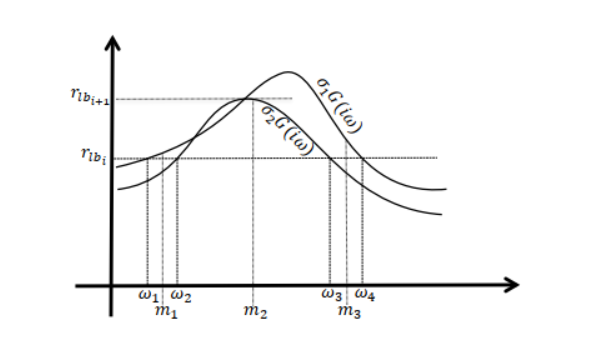
\includegraphics[width=13cm]{Anh3}
  \caption{Mỗi liên hệ giữa giá trị kỳ dị và giá trị riêng}
  \label{fig:pic3}
\end{figure}

Để bắt đầu thuật toán, ta đặt
\begin{align}\label{ct3.3.1}
    r_{lb} = max \left\{\sigma_{max}G(0), \sigma_{max}G(\omega_{p}i), \sigma_{max}(D)\right\}
\end{align}
để tìm cận dưới, trong đó $\omega_{p}$ = $\vert\ \lambda_{i}\vert$ và $\omega_{i}$ là cực của hàm truyền $G(s)$, được chọn theo tiêu chí sau:
\newline
Nếu hàm $G(s)$ có một hay nhiều cực là số ảo, thì $\lambda_i$ sẽ là cực làm cực đại hóa giá trị
\begin{align}\label{ct3.3.2}
    \abs{\frac{Im(\lambda_{i})}{Re(\lambda_{i})} \dfrac{1}{\lambda_{i}}}.
\end{align}
Nếu $G(s)$ có các cực hoàn toàn là số thực, thì $\lambda_{i}$ là cực làm cực đại hóa $\abs{\dfrac{1}{\lambda_{i}}}$.\\
Cũng như thuật toán phân đôi, phương pháp này áp dụng với hệ có ma trận A ổn định.

\begin{algorithm}[H]
\SetAlgoLined
\KwResult{Chuẩn \hinf}
\KwIn{Xét hệ \eqref{ct3.1.1} với các ma trận hệ số A, B, C, D. Trong đó ma trận A ổn định.}
Tính hàm truyền $G(s)$ của hệ.\\
Tìm các cực của $G(s)$.\\
\eIf{Các cực có giá trị thực chặt}{
    Đặt $\omega_p = max \abs{\lambda_{i}}$.
    }{
    Đặt $\omega_p = \lambda_{i}$, với $\lambda_{i}$ cực đại hóa \eqref{ct3.3.2}.
    }
    Tính $r_{lb}$ sử dụng công thức \eqref{ct3.3.1}.\\
    Tính $r = (1 + 2\epsilon)r_{lb}$.\\
    Tính $M_r$ bằng công thức \eqref{ct3.1.2}.
    Sắp xếp toàn bộ các giá trị thuần ảo của $M_r$, gán nhãn cho chúng theo chiều giảm dần từ $\omega_1, ... ,\omega_k.$
    Nếu $M_r$ không có giá trị thuần ảo nào, đặt $r_{ub} = r$ và chuyển sang bước 16.\\
    \For{$i\leftarrow 1$ \KwTo $k-1$} {
    (i) Tính $m_i$ = $\dfrac{1}{2}(\omega_i + \omega_{i+1})$.\\
    (ii) Tính $\omega_{max}(G(m_ii)) = svd_i$.\\
    Đặt $r_{lb} = max(svd_i)$.
    }
     Tính $\norm{G}_\infty = \dfrac{1}{2}(r_{lb} + r_{ub})$.
 \caption{Thuật toán hai bước}
\end{algorithm}

\newpage
Sau đây là đoạn mã thực thi thuật toán hai bước bằng ngôn ngữ Python.
\begin{lstlisting}[language=Python, caption=Thuật toán hai bước]
import numpy as np
from scipy.linalg import *
from control import *
from slycot import *

n = A.shape[0];
r = C.shape[0];
I = pow(A,0);
res = 0
temp1 = []
temp2 = []
e = 1e-6
tol = 1e-9

temp = signal.StateSpace(A,B,C,D);
sys = temp.to_ss()
G = sys.to_tf()
p = np.matrix.round(G.poles,6)

Wc = gram(sys,'c')
Wo = gram(sys,'o')

def is_stable(A):
    if np.any(np.linalg.eigvals(A).real >= 0.0):
        print("the system is unstable!")
    else: print("the system is stable!")

def find_pole(A):
  A_e_val=np.matrix.round(np.linalg.eigvals(A),6)
  w_p = 0
  if np.all(A_e_val.imag == 0):
    temp = max(abs(1/A_e_val[::]))
    for i in A_e_val:
      if(1/abs(i)==temp):
        w_p = max(abs(i))
    return w_p
  else:
    temp = max(abs((A_e_val[::].imag/A_e_val[::].real)*(1/A_e_val[::])))
    for i in A_e_val:
      if(abs((i.imag/i.real)*(1/i))==temp):
        w_p = i
    return w_p

def Hamil_matrix(A,B,C,D,q):
  M_r = np.zeros([2,2,n,n],dtype=np.complex)
  if np.all(D!=0):
    R = q**2*I - D.T*D
    M_r[0][0] = A + B*inv(R)*D.T*C
    M_r[0][1] = B*inv(R)*B.T
    M_r[1][0]= -C.T*(I + D*inv(R)*D.T)*C
    M_r[1][1]= -(A + B*inv(R)*D.T*C).T
    return np.matrix.round(M_r.transpose(0,2,1,3).reshape(6,6),6)
  else:
    M_r[0][0] = A
    M_r[0][1] = (1/q**2)*B*B.T
    M_r[1][0]= -C.T*C
    M_r[1][1]= -A.T
    return np.matrix.round(M_r.transpose(0,2,1,3).reshape(6,6),6)

w = round(abs(find_pole(A)),6)
def G(w):
  z = complex(0,w)
  return C*inv(z*I-A)*B + D

r_lb = round(max((max(svdvals(G(w)))),(max(svdvals(D))),max(svdvals(G(0)))),6)
r_ub = round(np.amax(svdvals(D)) + 2*np.sqrt(n*((Wc*Wo).trace())),6)

while (abs(r - r_lb)<=tol):
  r = (1+2*e)*r_lb
  H = Hamil_matrix(A,B,C,D,r)
  e_vals = eigvals(H)
  if np.all(e_vals.imag == 0):
    r_ub = r
    break
  else:
    i = 0
    while(i<len(e_vals)-1):
      sorted_eivals = -np.sort(-e_vals)
      m_i_dummy = 0.5*(sorted_eivals[i]+sorted_eivals[i+1])
      m_i = abs(m_i_dummy)
      temp1 = svdvals(G(m_i))
      svd_i = max(temp1)
      dummy = svd_i.tolist()
      temp2.append(dummy)
      i+=1
  r_lb = max(temp2)
  del temp2[:]
 
res = 0.5*(r_lb+r_ub) 
print(f'The solution is {res}')

System specification: Intel Core i7-4810MQ 2.8 GHz, 12GB RAM
\end{lstlisting}
Chuẩn \hinf được định nghĩa là giá trị kỳ dị cực đại trên trục ảo, nên ta có thể thử dọc theo trục ảo để tìm cận dưới cho chuẩn \hinf. Để có thể chắc chắn tính toán được $\norm{G(s)}_\infty$ bằng thuật toán hai bước, ta cần chọn cận dưới cho thuật toán một cách cẩn thận.
\newline
Sau khi tính các giá trị riêng của ma trận $M_r$, ta cần chọn xem $r$ làm cận trên hay dưới bằng cách sử dụng Định lý 2.1.1, tương tự thuật toán phân đôi. Tuy nhiên nếu ta tìm được các giá trị riêng thuần ảo $\omega_1, \omega_2,...,\omega_n$ thì theo Định lý 2.1.1, $r$ là giá trị kỳ dị với mỗi hàm $G(\omega_i)$. Điều này cho ta biết rằng có tồn tại các phản hồi $m_1, ..., m_{n-1}$, mỗi $m_i$ với hai điểm $\omega_i, \omega_{i+1}$ sẽ có một vài $m_i$ mà $G(\omega i) < G(m_i)$. Bằng cách tính $\sigma_{max}$ với $\forall$i, thuật toán hai bước tìm kiếm ở một khoảng rộng hơn nhiều với thuật toán phân đôi. Sau khi tìm $\sigma_{max}(G(m_i))$ với mọi i, ta đặt giá trị này bằng $r_{lb}$ và bắt đầu bước lặp tiếp theo.

\begin{example}
Có 
\newline
A = $\begin{bmatrix}
    -1.0000 + 1.0000i & -1.0000 & -1.0000\\
    -1.0000 & -2.0000 + 1.0000i & -1.0000\\
    -1.0000 & -1.0000 & -2.0000 - 1.0000i
\end{bmatrix}$.
\newline
Các cực của $G(s)$ là các giá trị riêng của A. Các giá trị đó là {-3.3589 + 0.2858i, -0.3628 + 0.9534i, -1.2784 - 0.2392i}. Vậy ma trận A ổn định.\\
Tiếp theo ta thấy -0.3628 + 0.9534i  cực đại hóa \eqref{ct3.3.2} và sử dụng \eqref{dly3.3.1} ta tính được $r_{lb}$ = 0.9907. Thực tế tính toán sẽ cho ra kết quả là 1.185206.\\
Sử dụng giá trị trên làm $r_{lb}$ ta đi tính,
\begin{align*}
M_r = 
\begin{bmatrix}
    -1 + i & -1 & -1 & 1.0188 & 0 & 0\\
    -1 & -2 + i & -1 & 0 & 0 & 0\\
    -1 & -1 & -2 - i & 0 & 0 & 0\\
    -1 & -1 & -1 & 1 + i & 1 & 1\\
    -1 & -1 & -1 & 1 & 2 + i & 1\\
    -1 & -1 & -1 & 1 & 1 & 2 - i  
\end{bmatrix}.
\end{align*}
Tính các giá trị riêng của $M_r$ ta được:
\begin{align*}
    -3.1927 + 0.2164\iu,\\
    3.1927 + 0.2164\iu,\\
    −1.3224 − 0.1563\iu,\\
    1.3224 − 0.1563\iu,\\
    −0.0000 + 0.8597\iu,\\
    0.0000 + 1.0201\iu.
\end{align*}
Ta tính và sắp xếp các giá trị riêng thuần ảo, $\omega_1$ = −0.0000 + 0.8597i và $\omega_2$ = 0.0000 + 1.0201i. Tính trung bình của 2 giá trị trên ta thu được $m_1$ = 0.0000 + 0.9399i.\\
Giá trị đơn lớn nhất của G($m_1i$) = 1.0121 = $r_{lb}$.\\
Ta tiếp tục chạy vòng lặp tiếp theo khi có các giá trị riêng chặt của $M_r$. Sau bốn vòng chạy, ta thu được $\norm{G}_\infty$ = 1.0121. Thực tế tính toán cho ra kết quả là 1.608108.
\end{example}
\bigskip
\begin{remark}
Ta thấy rằng một vấn đề chính nảy sinh trong việc triển khai thuật toán này là sự cần thiết của việc giải giá trị riêng chính xác, phụ thuộc vào việc các giá trị riêng thuần ảo hay không.
\end{remark}